\documentclass[../main.tex]{subfiles}

\begin{document}

\subsection{High-Level Overview}

\begin{figure}
	\centering
	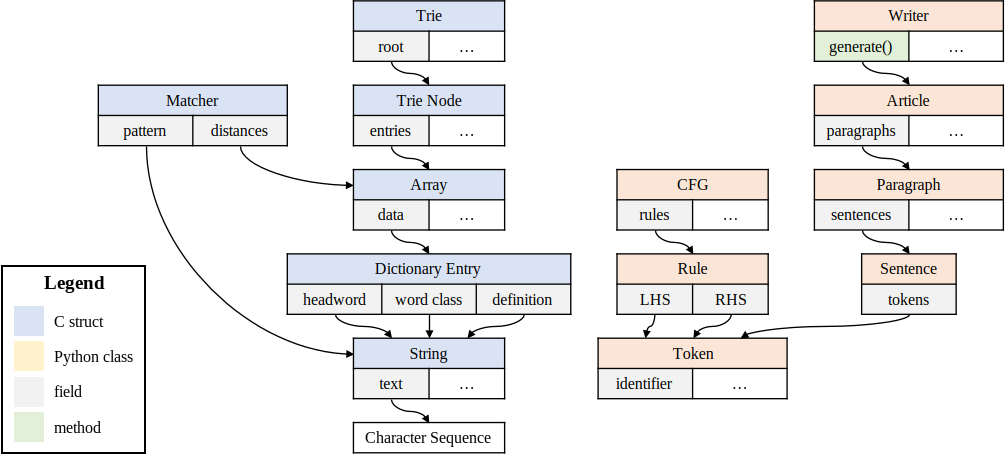
\includegraphics[scale=0.6]{project_structure}
	\caption{Overview of the project structure. Some fields and methods are omitted.}
	\label{figure:project_structure}
\end{figure}

\subsection{Languages}

I use C for the core dictionary because it runs faster and provides more precise memory control. I initially wrote it in Python, but it took 3 seconds to launch and violated the time constraint. The bottleneck turns out to be CPU computation as opposed to disk IO. Moving to C should effectively speed it up since compiled languages typically compute much faster than interpreted languages.

I use Python for the story writer because it is easier to code, supports regular expression and features various sampling methods. Usage of these functionalities is described in <Section>. Python libraries such as NumPy have a mature and efficient C/Fortran back-end. Compared to reinvented wheels, they are faster, more robust and easier to debug. Moreover, exception mechanism in Python makes it simpler to handle special cases that appear in a natural language.

\subsection{Data Structures}

\subsubsection{Dynamic Array}

Many functions in EngSci Press require a resizable and contiguous array. The most straightforward implementation is a block memory which is reallocated on each resize. However, frequent \texttt{realloc}s slow down the program. To make a trade-off between fewer \texttt{realloc}s and more compact storage, my custom \texttt{Array} type applies an exponential resizing strategy. It reserves more memory than its actual size. As shown in Figure \ref{figure:dynamic_array}, the memory space doubles when $\textrm{size} \geq \textrm{capacity}$ and halves when $\textrm{size} \leq \textrm{capacity} / 2$. A similar strategy is used for the \texttt{String} type.

\begin{figure}
	\centering
	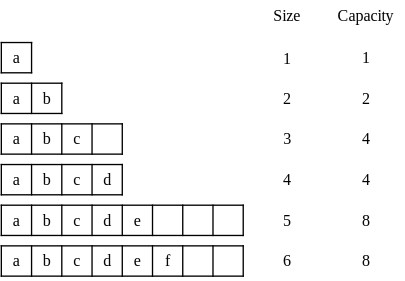
\includegraphics{dynamic_array}
	\caption{A dynamic array reserves space for future expansion.}
	\label{figure:dynamic_array}
\end{figure}

For convenience, an \texttt{Array} of pointers is designed to hold an optional destructor and execute it upon every element deletion. The destructor function frees all the memory that an element uses, both directly and indirectly.

\subsubsection{Trie}

I choose trie to store, access and modify dictionary data because it is efficient and easy to implement. Trie is a tree-like data structure that implements mapping with string keys. As shown in Figure \ref{figure:trie}, each node holds a single character. The key of a node is represented by the character sequence along the root-node path.

\begin{figure}
	\centering
	\includegraphics{trie}
	\caption{A trie. Each shadowed node represents an English word.}
	\label{figure:trie}
\end{figure}

Headwords are lower-cased as keys of dictionary entries, enabling case-insensitive search. Moreover, keys accept only characters whose ASCII codes fall in 32--64 or 97--122, because others are either upper-cased, or meaningless to appear in a dictionary headword. As a result, a trie node has 59 children at most.

For simplicity, mapping from a node to its children is implemented with a 59-element array of ordered child pointers. Fill \texttt{NULL} if a child does not exist. Such primitive implementation seems to hurt performance at first glance, as one has to check for many null pointers. However, because the accepted character set is small, a more advanced data structure, such as BST, usually brings more overhead as opposed to efficiency.

\subsubsection{Levenshtein Automaton}

\subsection{Software Implementation}

\subsubsection{Context-Free Grammar}

\subsubsection{Story Length Control}

\end{document}